\clearpage

\def\chaptertitle{Background}

\lhead{\emph{\chaptertitle}}

\chapter{\chaptertitle}
\label{ch:background}

In this chapter, a brief introduction to Service Level Agreements is provided in section \ref{sec:ch2-sla}, followed by an overview of micro-service architectures is provided in section \ref{sec:ch2-micro-svc-arc}. This includes a brief description of the architecture of Kubernetes, along with its scheduling and auto-scaling algorithms. Finally, a brief overview of time-series analysis is conducted in section \ref{sec:ch2-time-series}, along with some of the popular algorithms used.

\section{Service Level Agreements}
\label{sec:ch2-sla}

\begin{figure}[htb]
    \centering
    \caption{Overview of service level agreements}
    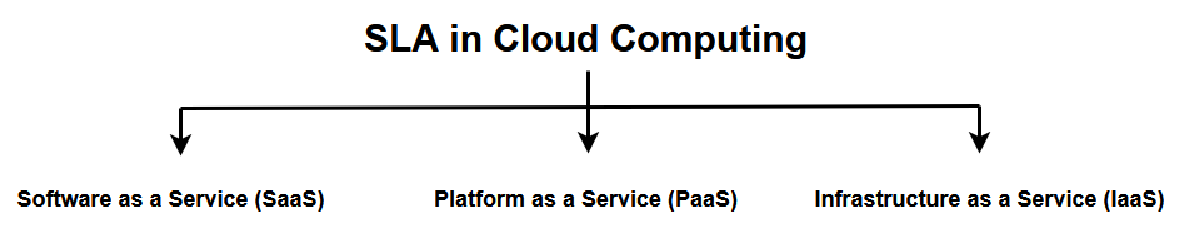
\includegraphics[width=0.9\linewidth]{Figures/SLA-Cloud-Computing.pdf}
    \label{fig:sla-types}
\end{figure}

Cloud computing generally exposes resource using a pay-as-you-go service. These lucrative plans have led to the implementation of applications and hardwares being delivered as Software as a Service (SaaS), Platform as a Service (PaaS), and Infrastructure as a Service (IaaS). However, consumers of such services have demands which may vary significantly, and it is impossible to fulfill all these expectations. Thus a balance needed to be struck in order to commit to an agreement \cite{patel2009service}. \par
This commitment is known as a Service Level Agreement (SLA). This SLA defines the expected services provided by the provider, and agreed to by the consumer. For example, one of the most common metric by which SLAs are negotiated between providers and consumers is the availability of service.

\subsection{Availability of Services}
\label{subsec:ch2-svc-availability}
Availability is defined to ensure that the functional performance of the edge deployment is maintained for an agreed period. SLAs mostly define either monthly or yearly downtime in order to compute service credits for billing purposes \cite{mirobi2015service}. The downtime can be calculated using the formulae:
%TC:ignore
\[ downtime_{monthly} = \frac{100 - Availability\%}{100} \times 30 \times 24 \]
\[ downtime_{yearly} = \frac{100 - Availability\%}{100} \times 365 \]
%TC:endignore
Table \ref{table:sla-availability} shows the expected down-times for several SLA availability percentages.

%TC:ignore
\begin{table}
    \caption{Summary of SLA availability}\label{table:sla-availability}
    \centering
    \begin{tabular}{|l|l|l|}
        \hline
        Availability \% & Monthly Downtime & Yearly Downtime\\
        \hline
        90\% & 72 hours & 36.5 days\\
        99\% & 7.2 hours & 3.65 days\\
        99.9\% & 43.8 minutes & 8.76 hours\\
        99.99\% & 4.38 minutes & 52.56 minutes\\
        99.999\% & 25.9 seconds & 5.26 minutes\\
        \hline
    \end{tabular}
\end{table}
%TC:endignore

\section{Microservice Architecture}
\label{sec:ch2-micro-svc-arc}

Micro-service architectures involve decomposing an application into several loosely coupled services, and deploying them on separate cloudlet servers known as ``nodes''. These services communicate with each other through a lightweight framework such as RESTful APIs \cite{li2021understanding}. Within these services, application data and commands are stored and executed within ``containers''. Typically, these architectures provide scalability, as well as ease of deployment and modification. Availability however, remains an important concern for such deployments. For a deployment to be classified as ``highly available'', it must be accessible at least 99.999\% of the time. For example, a highly available search engine would only face 5 minutes of down time per year \cite{nabi2016availability}. Therefore, an orchestration mechanism is required to manage the deployment and communication of these containers.\par

\begin{figure}[htb]
    \centering
    \caption{Features of container orchestration}
    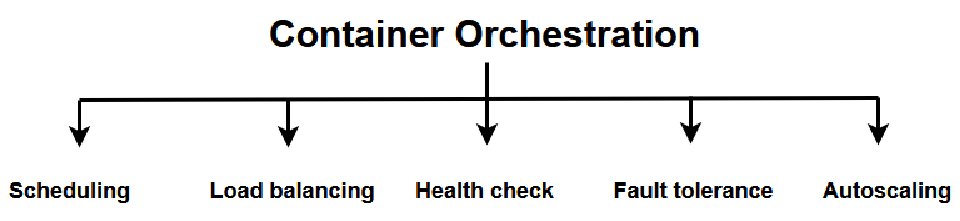
\includegraphics[width=0.9\linewidth]{Figures/Container-Orchestration.pdf}
    \label{fig:container-orchestration}
\end{figure}

Container orchestration allows the micro-service application to customize how the deployment, monitoring, and controlling functions \cite{casalicchio2019container}. Figure \ref{fig:container-orchestration} depicts the typical features of container orchestration.\par
\textit{Scheduling} defines the rules on the number of containers to be executed at any given time. Scheduling also places containers on specific nodes based on availability and best performance.\par
\textit{Load balancing} distributes the resource usage among multiple micro-service nodes. By default, a round-robin policy is implemented, although more complex policies may be implemented at the discretion of the developer.\par
\textit{Health checks} ensure that the container is still capable of responding to queries. Typically, these are done using a periodic light-weight HTTP request and verifying the response.\par
\textit{Fault tolerance} maintains several replicas of containers, a strategy commonly used to achieve the high availability mentioned above. Health checks are used to ensure the replicas are functioning, and they typically have strategies to ensure there is no mismatch in data between two fault tolerant containers.\par
\textit{Autoscaling} is the process of automatically adding or removing resources or containers. Internal metrics such as CPU usage are typically used, however custom policies can also be implemented at the discretion of the developer.\par

\subsection{Kubernetes Architecture}
\label{subsec:ch2-k8s-overview}

Kubernetes \footnote{\url{https://kubernetes.io/}} is one of the most popular open-source container orchestration platforms \cite{vayghan2019kubernetes}. Initially referred to as ``Borg'', the project was used internally at Google to deploy the majority of their cloud applications before becoming an open-source application \cite{burns2016borg}. Figure \ref{fig:k8s-arch} shows the high-level architecture. The Kubernetes deployment has a controller / worker architecture. The nodes in the Kubernetes cluster are split into either \textit{control plane nodes} and \textit{data plane nodes}. The \textit{control plane nodes} have a collection of processes which help monitor and maintain the desired state of the deployment. The \textit{data plane nodes} contain processes which run the containers doing the actual work, and are managed by the control plane.\par
The smallest unit of work in a Kubernetes deployment is known as a \textit{pod} \cite{baier2017getting}. This is a collection of containers sharing an IP address and port. In summary, micro-service architectures are said to be containerized and deployed on Kubernetes in the form of pods \cite{vayghan2019kubernetes}.\par
\begin{figure}[htb]
    \centering
    \caption{Overview of Kubernetes architecture}
    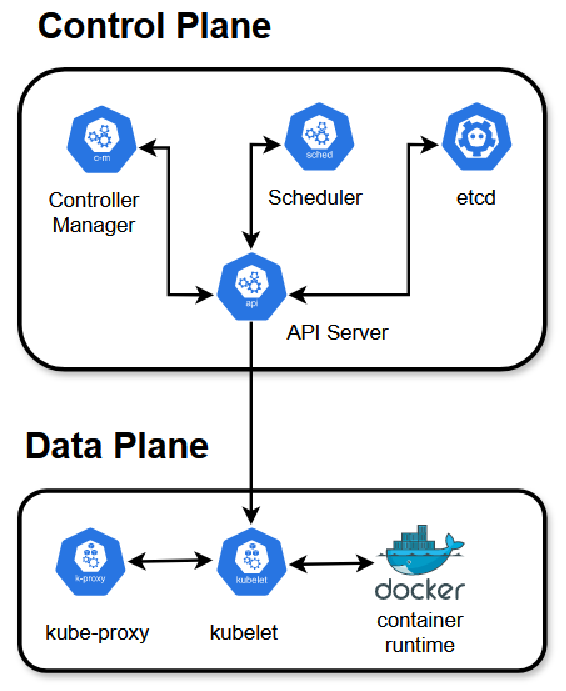
\includegraphics[width=0.5\linewidth]{Figures/K8s-Architecture.pdf}
    \label{fig:k8s-arch}
\end{figure}

\subsubsection{Control Plane}
\label{subsubsec:ch2-k8s-control-plane}
The \textit{API Server} is the primary communication endpoint for the entire deployment. Every component in the architecture communicates through it to exchange information. It is also used to update the current deployment state. The API Server is a simple RESTful API implementation, exposing well-documented APIs for access by other components as well as developers. Multiple replicas of this component are typically maintained to ensure high availability.\par

The \textit{etcd} is a data store which persists the deployment state in a key-value format. The data is serialized unlike in the stateless API server. This data adheres the properties of \textit{recovery} and \textit{availability}. \textit{Recovery} ensures that any corruption of data is reverted using a system of backups such as checkpoints. \textit{Availability} ensures that the deployment is reachable by the end-user regardless of the traffic being requested on the network.\par

\textit{Controller Manager} implements the desired deployment state. During initial deployment, the controller manager inputs the required workload as the desired state, after which it continually monitors the deployment state using a system of looping controls. If the deployment requires modifications, they are achieved using the API server, and the deployment is brought back into alignment with the desired state.\par

Finally, the \textit{scheduler} decides the location where the pod will be deployed. The scheduler runs a control loop which searches for unscheduled pods using the API server. It then assigns the pods to a dataplane node based on several predicates and priorities such as resource requirements and node affinity respectively.

\subsubsection{Data Plane}
\label{subsubsec:ch2-k8s-data-plane}

The \textit{container runtime} is a process which downloads or ``pulls'' the image for the required container onto the node. Kubernetes supports a wide range of runtimes, but some of the popular solutions are CRI-O \footnote{\url{https://cri-o.io/}}, containerd \footnote{\url{https://containerd.io/}}, and Docker \footnote{\url{https://www.docker.com/}}.\par

The most important process running on every data plane node is the \textit{kubelet}. This process executes the image assigned to the node via the container runtime, perform health checks, and reports the node status to the control plane.\par

Another data plane process is the \textit{kube-proxy}, which manages the rules for forwarding requests to services, as well as the IP tables of nodes. If a service is added or removed, kube-poxy updates the IP table accordingly.\par

\section{Auto-scaling Overview}
\label{sec:ch2-auto-scaling}

Apart from intelligently scheduling pods to data plane nodes, Kubernetes has the provisions to dynamically respond to changes in resource requirements \cite{kayal2020kubernetes}. This process of scaling nodes, pods, or other resources depending on requirements in an automated manner is known as \textit{auto-scaling}. Kubernetes supports three variations of auto-scaling.\par

\textit{Cluster auto-scaling} modifies the number of nodes running in the entire deployment, or cluster. Dynamically allocating nodes based on resource requirements helps to manage the cost of running Kubernetes deployments on external platforms such as Amazon \footnote{\url{https://docs.aws.amazon.com/eks/}} or Google \footnote{\url{https://cloud.google.com/kubernetes-engine/}}. The autoscaler works by looping through two tasks. The first watches for unscheduled pods, the second checks if the current deployed pods (pods which are running on the data plane) can be merged on a smaller number of nodes.\par

\textit{Vertical pod auto-scaling} modifies the CPU and memory resources assigned to pods. By default, the scheduler reserves a larger amount of these resources to pods than is usually required. By performing vertical pod auto-scaling, the cluster can better manage its over-provisioned resources in real-time.\par

\textit{Horizontal pod auto-scaling} is the most commonly used auto-scaling strategy \cite{baresi2021kosmos}. It modifies the number of pods assigned to a task, based on the resources being requested. Kubernetes implements this using a periodic control loop which runs every 15 seconds by default. The control manager compares the actual resource utilization with the target utilization defined by the deployment script, and scales the number of pods accordingly.

\subsection{Custom Auto-scaling}
\label{subsec:ch2-custom-auto-scaling}

The default horizontal pod autoscaler uses pod CPU and memory utilization when making its scaling decisions. However, these metrics may be too rigid when it comes to scaling edge architecture resources \cite{coulson2020adaptive}. The strict SLA constraints in place, along with the lower amount of resources present in the edge layer as compared to the cloud layer, make it imperative for custom metrics to be employed to autoscale resources as efficiently as possible.\par

Figure \ref{fig:custom-autoscale-overview} depicts the general architecture of the custom autoscaler. Typically, the autoscaler queries metrics from the default metrics registry, which acts as a central store for all metrics that are exposed to the developer. Three interfaces to this registry are exposed:
\begin{itemize}
    \item \textit{Resource metric API} is used to access predefined metrics such as CPU and memory resources of both pods as well as nodes.
    \item \textit{Custom metric API} contains user-defined custom metrics associated with all Kubernetes objects.
    \item \textit{External metrics API} contains metrics of objects which are not associated with Kubernetes.
\end{itemize}
For custom metric auto-scaling, the autoscaler must be configured in a way where the metrics can be fetched from the custom metric API. This is done by configuring the custom metric server, several frameworks to simplify this process such as the Kubernetes Instrumentation SIG \footnote{\url{https://github.com/kubernetes/community/tree/master/sig-instrumentation}} exist which simplify the server building process.

\begin{figure}[htb]
    \centering
    \caption{Custom autoscaler architecture overview.}
    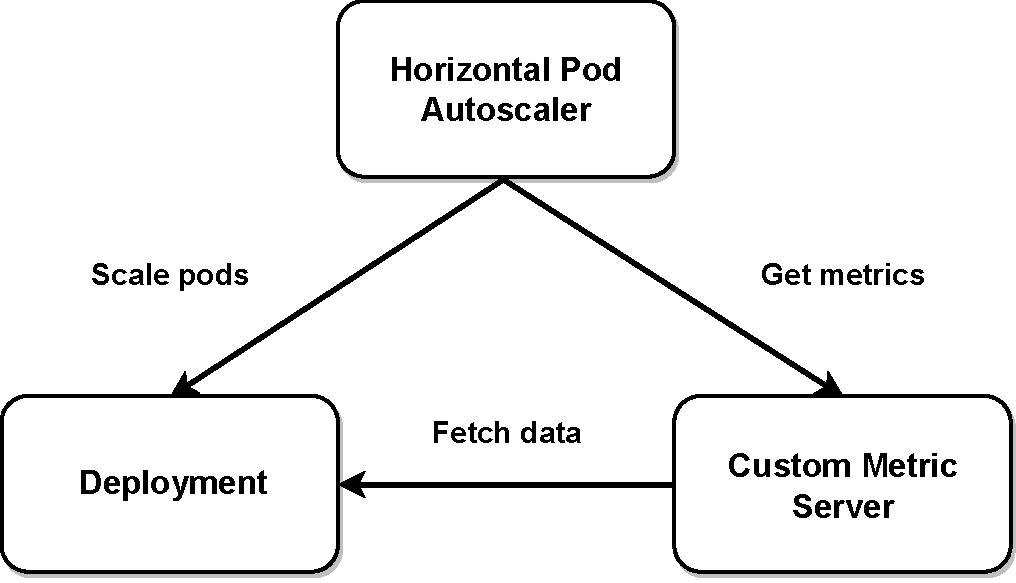
\includegraphics[width=.7\linewidth]{Figures/Custom-Metrics-Autoscaling.pdf}
    \label{fig:custom-autoscale-overview}
\end{figure}

\section{Time-Series Analysis}
\label{sec:ch2-time-series}

Several machine learning algorithms exist, however not all of them are suitable for time-series analysis \cite{mahmoud2021survey}. One of the most popular traditional models is the Convolutional Neural Network (CNN), which is a form of deep learning that attempts to learn data features through the process of filters being applied to the input at each convolutional layer, and the output being passed to the next layer. However, while CNNs are excellent when working with 3-dimensional data such as images, it does not perform well when dealing with sequential inputs with interdependent data \cite{zhao2017convolutional}. Due to this, another machine learning subset known as Recurrent Neural Network (RNN) was conceptualized. \par

\subsection{Architecture Overview}
\label{subsec:ch2-time-series-overview}

Recurrent Neural Networks store information about the past, and its future decisions are based on this information. Thus, while RNNs have a similar training process as CNNs, they remember features learned from prior inputs. RNNs are recurrent since they perform the same computation for each data element in the sequence, with each output being dependent on the previous computation. Figure \ref{fig:rnn-architecture} depicts this high-level architecture of the RNN.\par

\begin{figure}[htb]
    \centering
    \caption{Recurrent Neural Network architecture}
    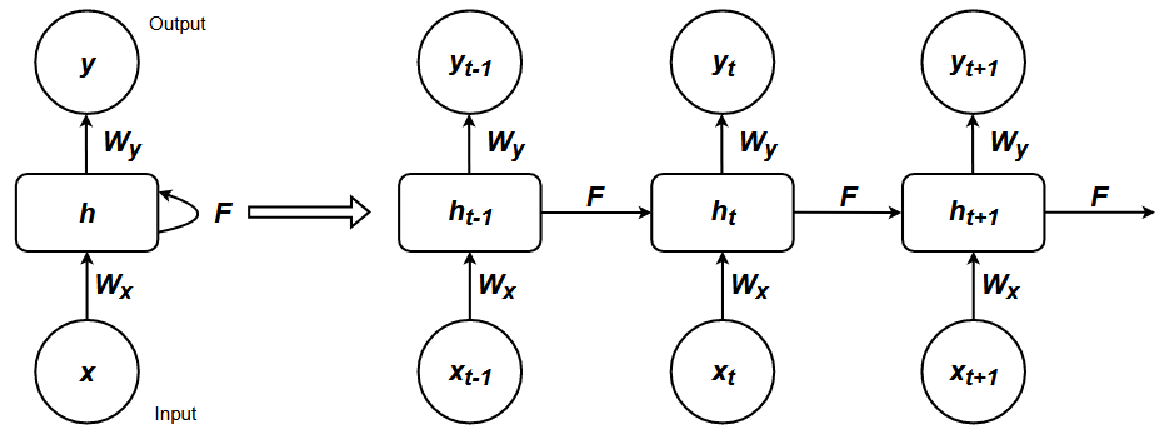
\includegraphics[width=1.0\linewidth]{Figures/RNN-Overview.pdf}
    \label{fig:rnn-architecture}
\end{figure}

For the current RNN state, the formula can be written as follows:

\begin{equation}
    h_{t} = \mathcal{F}(h_{t-1}, x_{t})
\end{equation}

Where $h_{t}$ is the current state, $h_{t-1}$ is the previous state, and $x_{t}$ is the current input value. In the simplest form, the function $\mathcal{F}$ is the activation function. Thus using the recurrent neuron weight $W_{h}$ and input weight $W_{x}$, the equation can be re-written as:

\begin{equation}
    h_{t} = \tanh(W_{h}h_{t-1} + W_{x}x_{t})
\end{equation}

Using this current state value, the output can be calculated using the equation:

\begin{equation}
    y_{t} = W_{y}h_{t}
\end{equation}

Where $W_{y}$ is the output weight.\par

RNN also employs a back-propagation algorithm during training. However, the parameters are used by all the network states $h_{i}; i \in \{1, 2, ... , n\}$. However, RNN training encounters two big issues, namely the vanishing and exploding gradients. These issues hinder the accuracy of predictions. If the training sequence is too long, the RNN has a difficult time carrying previous information from one training iteration to the next. To address this issue, an improved version of RNNs was created, known as LSTM.\par

Long Short-Term Memory or LSTM is a deep learning model which is enhanced from the traditional RNN architecture \cite{lindemann2021survey}. In an RNN function, the hidden state activation is influenced by nearby activation functions. This is known as the ``short-term'' memory. Meanwhile the overall network weights are influenced by the computations which occur over the entire long data sequence.\par

\begin{figure}[htb]
    \centering
    \caption{LSTM cell architecture}
    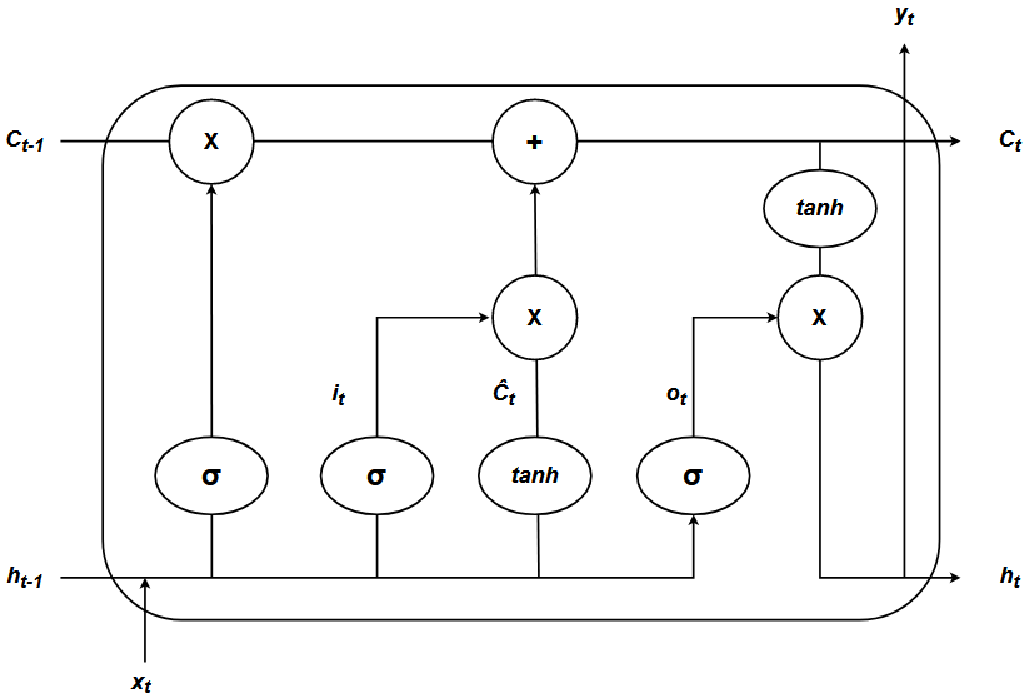
\includegraphics[width=0.8\linewidth]{Figures/LSTM-Cell-Architecture.pdf}
    \label{fig:lstm-cell-architecture}
\end{figure}

LSTMs are designed in a way which avoids the long-term dependency problem by integrating a cell state into the architecture. The cell state acts as a conveyor belt of information, allowing information to be passed along the different data sequences easily. Information is added to or removed from the cell state using structures known as gates. These gates are created from a sigmoid layer, and a point-wise multiplication operation. The LSTM architecture has three gates for performing cell state operations. These are the ``Forget gate'', ``Input gate'', and ``Output gate''. Figure \ref{fig:lstm-cell-architecture} shows the structure of these cell state operations.\par

The forget gate determines the amount of past information the LSTM should retain. This decision is made through the use of a sigmoid function, and the gate output $f_{t}$ is given through the equation:

\begin{equation}
    f_{t} = \sigma(W_{f}\cdot[h_{t-1}, x_{t}] + b_{f})
\end{equation}

Where $W$ is the gate neuron weight, and $b_{x}$ is the gate bias.\par

The input gate determines how information is added to the cell state. This is done through the following steps:
\begin{itemize}
    \item Determine the values $i_{t}$ to be added:
    \begin{equation}
        \label{eqn:input-gate}
        i_{t} = \sigma(W_{i}\cdot[h_{t-1}, x_{t}] + b_{i})
    \end{equation}
    \item Create vector $\hat{C_{t}}$ of all the possible values that may be added:
    \begin{equation}
        \hat{C_{t}} = \tanh( W_{C}\cdot[h_{t-1}, x_{t}] + b_{C})
    \end{equation}
    \item Use the computed value and vector, along with the previous cell state $C_{t-1}$ to obtain the useful information which can be added to current cell state $C_{t}$:
    \begin{equation}
        C_{t} = f_{t} \times C_{t-1} + i_{t} \times \hat{C_{t}}
    \end{equation}
\end{itemize}

Finally, the output gate determines which portion of the current cell state is included in the output. This is determined using three steps:
\begin{itemize}
    \item Create vector $o_{t}$ which scales the cell state value between -1 and +1:
    \begin{equation}
        \hat{C_{t}} = \tanh(C_{t})
    \end{equation}
    \item Compute filter value $o_{t}$ which regulates which values from $o_{t}$ are included in the output:
    \begin{equation}
        o_{t} = \sigma( W_{o}\cdot[h_{t-1}, x_{t}] + b_{o})
    \end{equation}
    \item Multiply the vector and filter to get the output $h_{t}$ which also acts as the hidden state of the next cell:
    \begin{equation}
        h_{t} = o_{t} \times \hat{C_{t}}
    \end{equation}
\end{itemize}

\subsection{Forecast Models}
\label{subsec:ch2-time-series-forecast-models}

There are two major methods of using a time-series model to determine the predicted outcomes, namely a one-step forecast model, and a multi-step forecast model.\par

In a \textit{One Step Forecast}, the time-series model first extracts short-term characteristics and correlations amongst the variables. It then feeds these into the various layers of its architecture during the training process, and finally generates a point forecast. In theory, such an approach would be more efficient, however it is heavily dependant on the correct training specifications and hyper-parameter selections, and thus is difficult to configure \cite{marcellino2006comparison}.\par

In a \textit{Multi Step Forecast}, the time-series model does the same training steps as the above approach, but then it predicts several data points of output in one single shot. Such an approach may take less time to make a prediction, and has less chances of inaccurate predictions due to it being more robust to model misspecifications.
